\documentclass[border=1pt]{standalone}
% Shared preamble for standalone figures in this directory.
% Compile with XeLaTeX from 讲义/figs, or via the figures target.
\usepackage{ctex}
\usepackage{amsmath}
\usepackage{amssymb}
\usepackage{bm}
\usepackage{mathtools}
\usepackage{tikz}
\renewcommand{\vec}[1]{\boldsymbol{#1}}
\newcommand{\cC}{\mathcal{C}}
\newcommand{\cD}{\mathcal{D}}
\newcommand{\R}{\mathbf{R}}
\usetikzlibrary{
    arrows.meta,
    calc,
    decorations.markings,
    angles,
    quotes,
    positioning,
    patterns,
    shapes.geometric
}

\begin{document}
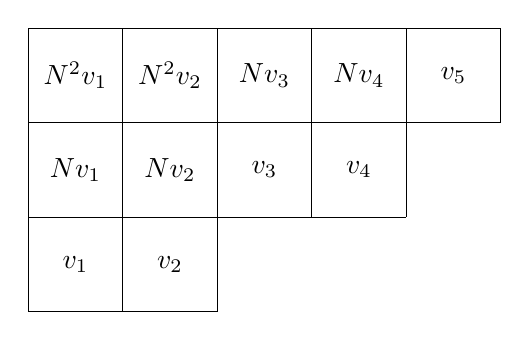
\begin{tikzpicture}[scale=1.2]
    \foreach[count=\i] \len in {5, 5, 4, 2}
    \draw (0, -\i+1) -- (\len, -\i+1);

    \foreach \i in {0,...,5}
    \draw (\i, 0) -- (\i, -1);
    \foreach \i in {0,...,4}
    \draw (\i, -1) -- (\i, -2);
    \foreach \i in {0, 1, 2}
    \draw (\i, -2) -- (\i, -3);

    \node at (.5, -.5) {$N^2v_1$};
    \node at (1.5, -.5) {$N^2v_2$};
    \node at (2.5, -.5) {$Nv_3$};
    \node at (3.5, -.5) {$Nv_4$};
    \node at (4.5, -.5) {$v_5$};
    \node at (.5, -1.5) {$Nv_1$};
    \node at (1.5, -1.5) {$Nv_2$};
    \node at (2.5, -1.5) {$v_3$};
    \node at (3.5, -1.5) {$v_4$};
    \node at (.5, -2.5) {$v_1$};
    \node at (1.5, -2.5) {$v_2$};
\end{tikzpicture}

\end{document}
